\documentclass{beamer}
\usetheme{Madrid}
\usepackage[utf8]{inputenc}
\usepackage[portuguese]{babel}
\usepackage{booktabs}

\title[Previsão de Notas]{Previsão de Notas de Review (Olist)}
\subtitle{Introdução à Ciência de Dados — NES}
\author{Tiago Cavalcante Trindade}
\date{Julho de 2025}

\begin{document}

% ------------------------------------------------
\begin{frame}
  \titlepage
\end{frame}

% ------------------------------------------------
\begin{frame}{Problema}
  \begin{itemize}
    \item Prever a \textbf{review\_score} (1-5 estrelas) antes do cliente avaliar.
    \item Base de dados pública da \textbf{Olist}.
    \item \textbf{Features}
          \begin{itemize}
            \item Numéricas: tempo de entrega, valor do carrinho, frete, nº de itens, pagamentos, dia da semana, mês.
            \item Texto: título + mensagem da review $\rightarrow$ vetor FastText spaCy (300 dim) $\rightarrow$ SVD (120 dim).
          \end{itemize}
    \item Balanceamento por undersampling; divisão temporal 80/20 (treino/teste).
  \end{itemize}
\end{frame}

% ------------------------------------------------
\begin{frame}{Modelos Avaliados}
  \begin{enumerate}
    \item Regressão Linear (arredondada \& cortada)
    \item Regressão Logística Multiclasse
    \item Regressão Logística Ordinal
  \end{enumerate}
  Implementados com \texttt{scikit-learn} (+ \texttt{mord} para o modelo ordinal).
\end{frame}

% ------------------------------------------------
\begin{frame}{Matrizes de Confusão}
  \centering
  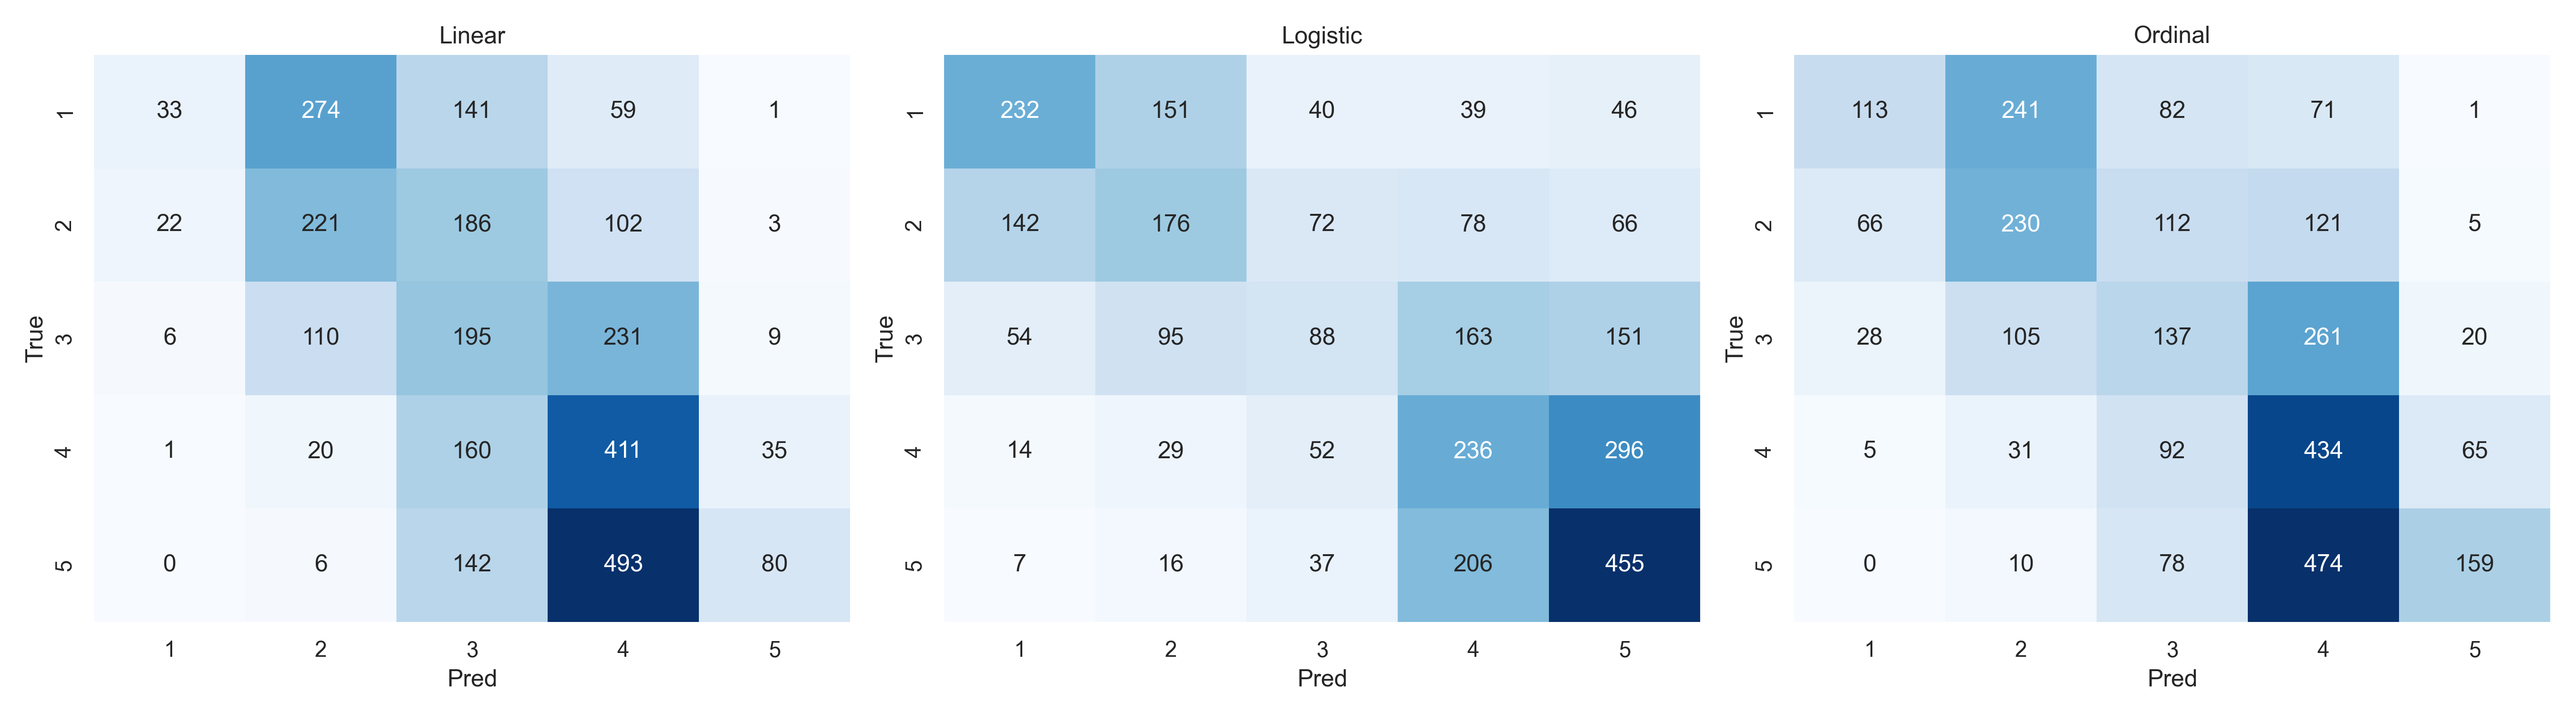
\includegraphics[width=0.95\linewidth]{../figures/confusion_matrices.png}
\end{frame}

% ------------------------------------------------
\begin{frame}{Acurácia por Modelo}
  \centering
  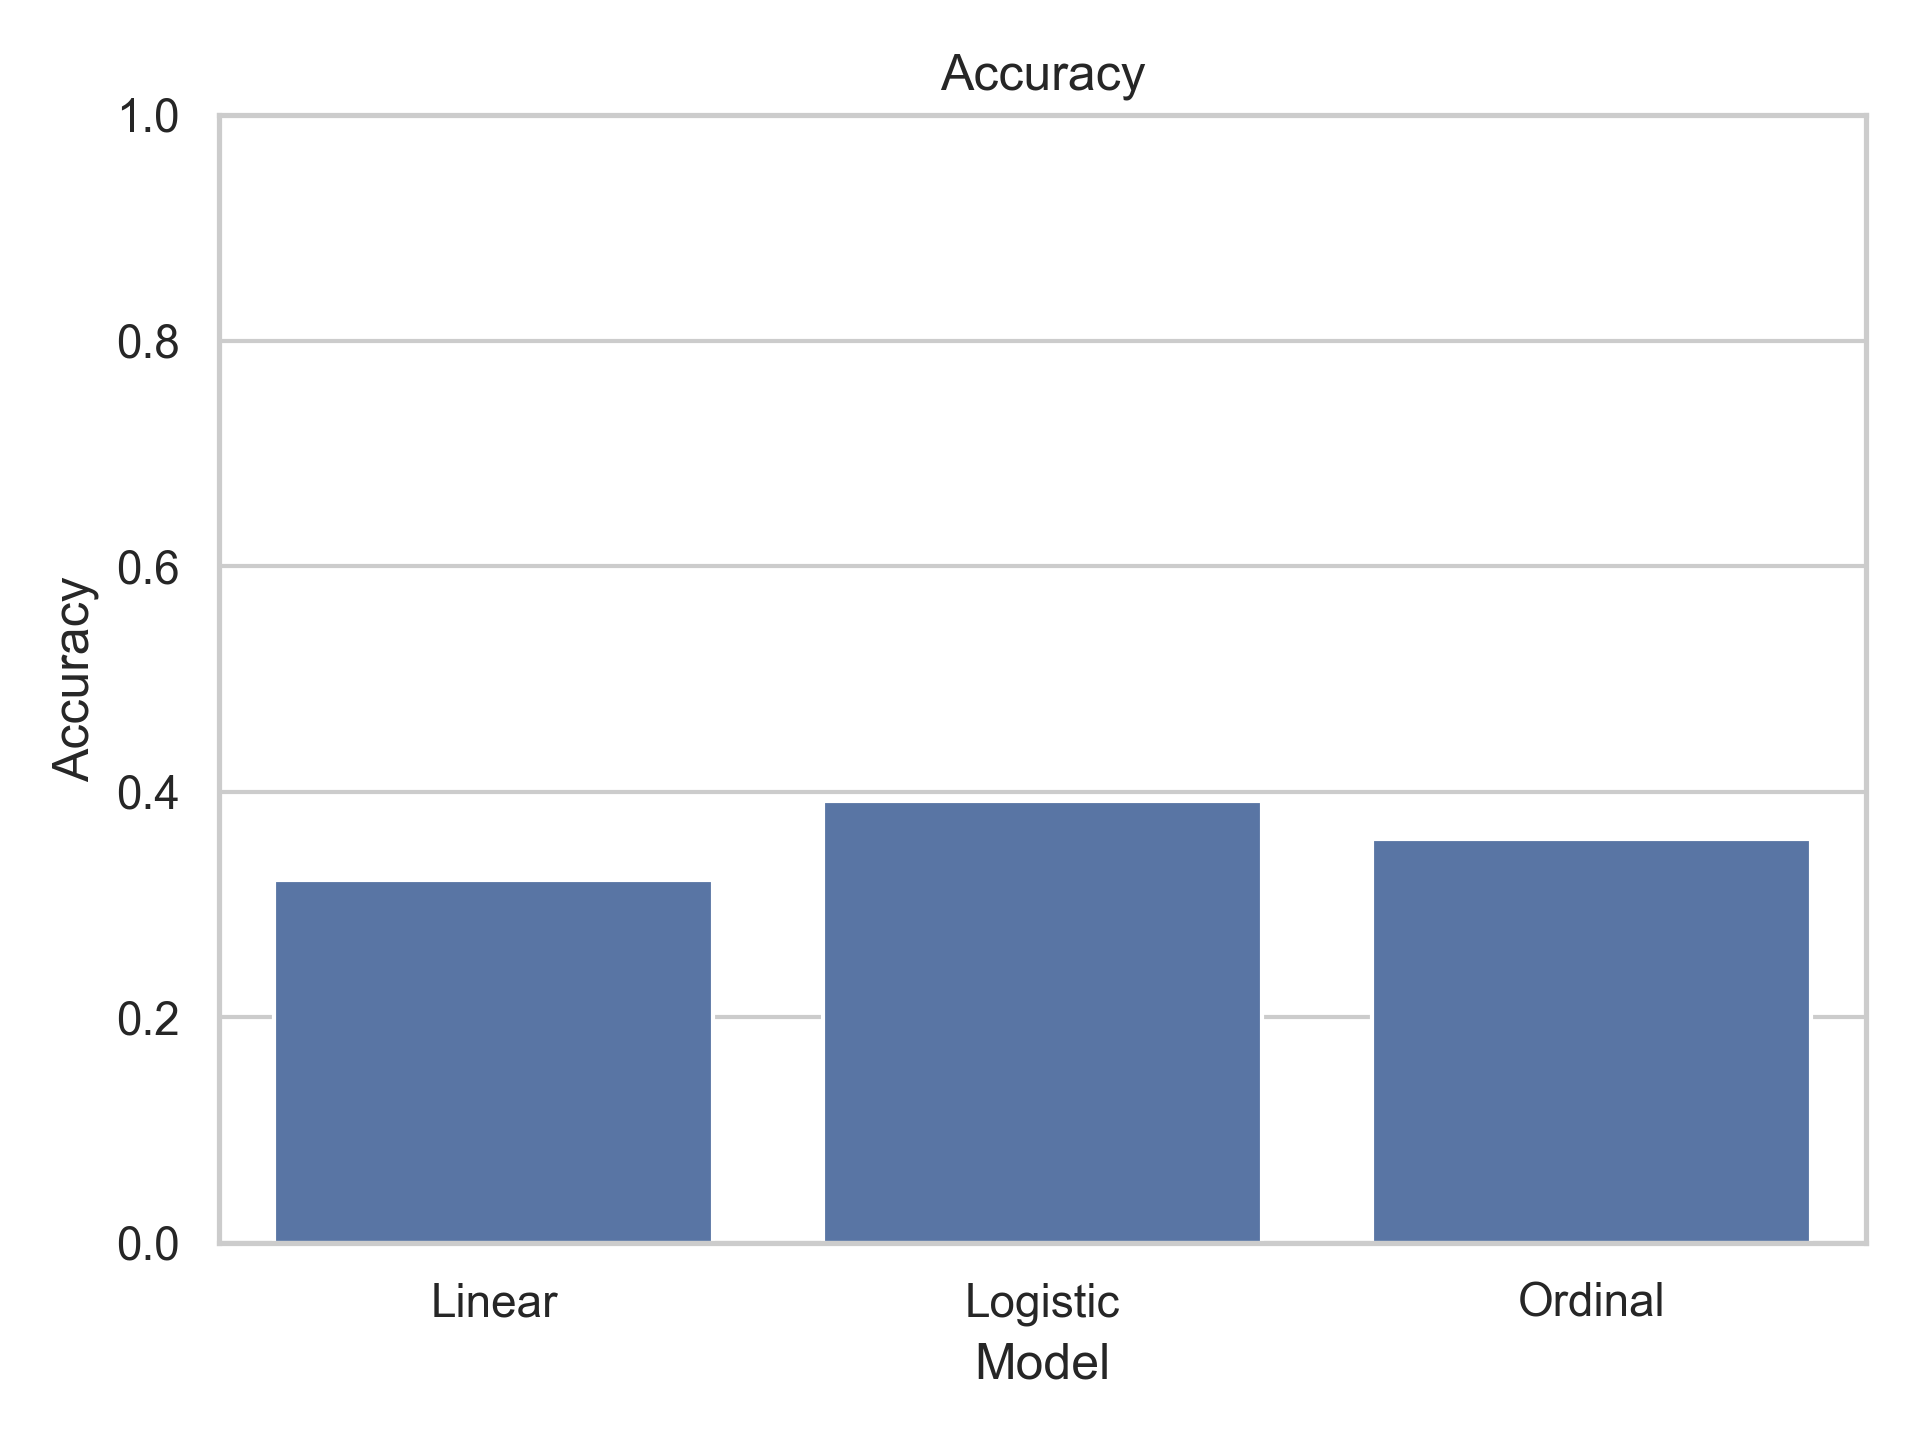
\includegraphics[width=0.55\linewidth]{../figures/accuracy.png}
\end{frame}

% ------------------------------------------------
\begin{frame}{Resumo de Métricas}
  \footnotesize
  \begin{table}[h]
    \centering
    \begin{tabular}{lccc}
      \toprule
      \textbf{Modelo}             & \textbf{Acurácia} & \textbf{MAE}   & \textbf{RMSE}  \\
      \midrule
      Regressão Linear (arred.)   & 0.321             & 0.917          & \textbf{1.105} \\
      Regr. Logística Multiclasse & \textbf{0.391}    & 0.882          & 1.263          \\
      Regr. Logística Ordinal     & 0.358             & \textbf{0.823} & 1.115          \\
      \bottomrule
    \end{tabular}
  \end{table}
\end{frame}

% ------------------------------------------------
\begin{frame}{Principais Insights}
  \begin{itemize}
    \item Logística Multiclasse: melhor acerto exato (aproximadamente 40\%).
    \item Logística Ordinal: menor MAE e RMSE — erra geralmente só \(\pm 1\) estrela.
    \item Regressão Linear é apenas um baseline simples.
  \end{itemize}
\end{frame}

% ------------------------------------------------
\begin{frame}{Conclusão}
  \begin{block}{Escolha}
    \begin{itemize}
      \item Se o KPI exige acerto exato da nota \(\Rightarrow\) \textbf{Logística Multiclasse}.
      \item Se o mais importante é limitar a distância do erro \(\Rightarrow\) \textbf{Logística Ordinal}.
    \end{itemize}
  \end{block}
\end{frame}

\end{document}
